\ifdefined\included
\else
\documentclass[french, a4paper, 11pt, twoside, pdftex]{StyleThese}
\usepackage{iflang}
\usepackage{bibentry}



%\usepackage[sectionbib]{chapterbib}          % Cross-reference package (Natural BiB)
%\usepackage{natbib}                  % Put References at the end of each chapter
%\usepackage{bibunits}
% Do not put 'sectionbib' option here.
% Sectionbib option in 'natbib' will do.


\usepackage{fancyhdr}                    % Fancy Header and Footer

\usepackage[utf8]{inputenc}
\usepackage[T1]{fontenc}
\usepackage[french]{babel} %
\usepackage{lmodern} \normalfont %to load T1lmr.fd 
\DeclareFontShape{T1}{cmr}{b}{sc} { <-> ssub * cmr/bx/sc }{}
%\hyphenation{gar}

\usepackage{amsmath,amssymb}             % AMS Math
\usepackage{nicefrac}
\usepackage{siunitx}					%% Unites Math SI

\usepackage{blindtext}

\usepackage{datetime}

\usepackage{lipsum} 

\usepackage[inline]{enumitem}

\usepackage{hhline}
%\usepackage[left=1.5in,right=1.3in,top=1.1in,bottom=1.1in]{geometry}
\usepackage[left=1.5in,right=1.3in,top=1.1in,bottom=1.1in,includefoot,includehead,headheight=13.6pt]{geometry}

%%\renewcommand{\baselinestretch}{1.05}

%%%%%%%% Multi-figures avec sub-captions
\usepackage{caption}
\usepackage{subcaption}

% Table of contents for each chapter

\usepackage[nottoc, notlof, notlot]{tocbibind}
\usepackage[nohints]{minitoc}
\setcounter{minitocdepth}{2}
\mtcindent=15pt
% Use \minitoc where to put a table of contents

\usepackage{aecompl}

%% Package cosmetic meilleur layout du texte en jouant sur le spacing par caractères
\usepackage[activate={true,nocompatibility},final,tracking=true,kerning=true,factor=1100,stretch=10,shrink=10]{microtype}
\usepackage[absolute,overlay]{textpos} 
\setlength{\TPHorizModule}{\paperwidth}\setlength{\TPVertModule}{\paperheight}
\sloppy

%%%%%%%%%%% JOLIS TABLEAUX
\usepackage{tabularx}		%\usepackage{tabular}
\usepackage{longtable}
\usepackage{multirow}
\newcommand{\mc}{\multicolumn} 
\newcommand{\mr}[2]{\multirow{#1}{*}{#2}} 	\newcommand{\mrQ}{\multirow{-4}{*}}
\usepackage{booktabs}

\usepackage[usenames,dvipsnames]{xcolor} 

\makeatletter
\newcommand{\ccolor}[3][]{%
	\kern-\fboxsep
	\if\relax\detokenize{#1}\relax
	\expandafter\@firstoftwo
	\else
	\expandafter\@secondoftwo
	\fi
	{\colorbox{#2}}%
	{\colorbox[#1]{#2}}%
	{#3}\kern-\fboxsep
}
\makeatother

%%%%% Insertion graphiques format PGF
\usepackage{pgfplots}
\pgfplotsset{width=\linewidth, compat=1.16}%, compat=1.17}
\usepackage{adjustbox}          %%% PERMET DE LES RECADRER + FACILEMENT


%%%%%%%%%% Bullets de listes sans saut de ligne %%%%%%%%%%
\usepackage{xparse}

\ExplSyntaxOn%
\seq_new:N \l_local_enum_seq

\newcommand{\storethestuff}[1]{%
  \seq_set_from_clist:Nn \l_local_enum_seq {#1}%
}

\newcommand{\dotheenumstuff}{%
\int_zero:N \l_tmpa_int
\seq_map_inline:Nn \l_local_enum_seq {%
    \int_incr:N \l_tmpa_int% Increase the counter
    \item ##1
    % Check whether the list has reached the end -- if so, use '.' instead of ','
    %\int_compare:nNnTF 
    % { \l_tmpa_int } < {\seq_count:N \l_local_enum_seq} 
    % {,} {.}
  }
}
\ExplSyntaxOff

\NewDocumentCommand{\linebullets}{+m}{%
  \storethestuff{#1}%
  \begin{enumerate*}[label={\alph*)},font={\bfseries},itemjoin={{, }}]
    \dotheenumstuff%
  \end{enumerate*}
}

\newcommand{\cmnt}[1]{}  %%%%% AJOUT DE COMMENTAIRE MULTILIGNES


%%%%%%%%%% ECRITURE CARACTERES DANS UN CERCLE %%%%%%%%%%
%\def\circleTxt[#1]{\raisebox{.5pt}{\textcircled{\raisebox{-1pt}{#1}}}}
\newcommand{\ctxt}[1]{\raisebox{.5pt}{\textcircled{\raisebox{-1.2pt}{#1}}}}
% Glossary / list of abbreviations

\usepackage[intoc]{nomencl}
\IfLanguageName{english}{%
\renewcommand{\nomname}{Glossary}
}{ %
\renewcommand{\nomname}{Liste des Abréviations}
}

\makenomenclature

% My pdf code

\usepackage{ifpdf}

\ifpdf
  \usepackage[pdftex]{graphicx}
  \DeclareGraphicsExtensions{.pdf,PDF,.png,PNG,.jpg,JPG}
  \usepackage[pagebackref,hyperindex=true]{hyperref} %% use \autoref{} instead of Table~\ref{}.
  \usepackage{tikz}
  \usetikzlibrary{arrows,shapes,calc}
\else
  \usepackage{graphicx}
  \DeclareGraphicsExtensions{.ps,.eps}
  \usepackage[a4paper,dvipdfm,pagebackref,hyperindex=true]{hyperref}
\fi

\graphicspath{{.}{schemas/}{graphiques/}{tables/}}

%% nicer backref links. NOTE: The flag ThesisInEnglish is used to define the
% language in the back references. Read more about it in These.tex

\IfLanguageName{english}{
\renewcommand*{\backref}[1]{}
\renewcommand*{\backrefalt}[4]{%
\ifcase #1 %
(Not cited.)%
\or
(Cited in page~#2.)%
\else
(Cited in pages~#2.)%
\fi}
\renewcommand*{\backrefsep}{, }
\renewcommand*{\backreftwosep}{ and~}
\renewcommand*{\backreflastsep}{ and~}
}{
\renewcommand*{\backref}[1]{}
\renewcommand*{\backrefalt}[4]{%
\ifcase #1 %
(Non cité.)%
\or
(Cité en page~#2.)%
\else
(Cité en pages~#2.)%
\fi}
\renewcommand*{\backrefsep}{, }
\renewcommand*{\backreftwosep}{ et~}
\renewcommand*{\backreflastsep}{ et~}
}

% Links in pdf
\usepackage{color}
\definecolor{linkcol}{rgb}{0,0,0.4} 
\definecolor{citecol}{rgb}{0.5,0,0} 
\definecolor{linkcol}{rgb}{0,0,0} 
\definecolor{citecol}{rgb}{0,0,0}
% Change this to change the informations included in the pdf file

\hypersetup
{
bookmarksopen=true,
pdftitle="Prévention des fautes temporelles sur architectures multicœur pour les systèmes à criticité mixte",
pdfauthor="Daniel LOCHE", %auteur du document
pdfsubject="Thèse", %sujet du document
%pdftoolbar=false, %barre d'outils non visible
pdfmenubar=true, %barre de menu visible
pdfhighlight=/O, %effet d'un clic sur un lien hypertexte
colorlinks=true, %couleurs sur les liens hypertextes
pdfpagemode=UseNone, %aucun mode de page
%pdfpagelayout=DoublePage, %ouverture en simple page
pdffitwindow=true, %pages ouvertes entierement dans toute la fenetre
linkcolor=linkcol, %couleur des liens hypertextes internes
citecolor=citecol, %couleur des liens pour les citations
urlcolor=linkcol %couleur des liens pour les url
}

% definitions.
% -------------------

\setcounter{secnumdepth}{3}
\setcounter{tocdepth}{2}

% Some useful commands and shortcut for maths:  partial derivative and stuff

\newcommand{\pd}[2]{\frac{\partial #1}{\partial #2}}
\def\abs{\operatorname{abs}}
\def\argmax{\operatornamewithlimits{arg\,max}}
\def\argmin{\operatornamewithlimits{arg\,min}}
\def\diag{\operatorname{Diag}}
\newcommand{\eqRef}[1]{(\ref{#1})}
\newcommand{\nline}{\smallbreak\noindent}

\usepackage{rotating}                    % Sideways of figures & tables

% \usepackage{txfonts}                     % Public Times New Roman text & math font
  
%%% Fancy Header %%%%%%%%%%%%%%%%%%%%%%%%%%%%%%%%%%%%%%%%%%%%%%%%%%%%%%%%%%%%%%%%%%
% Fancy Header Style Options

\pagestyle{fancy}                       % Sets fancy header and footer
\fancyfoot{}                            % Delete current footer settings

%\renewcommand{\chaptermark}[1]{         % Lower Case Chapter marker style
%  \markboth{\chaptername\ \thechapter.\ #1}}{}} %

%\renewcommand{\sectionmark}[1]{         % Lower case Section marker style
%  \markright{\thesection.\ #1}}         %

\fancyhead[LE,RO]{\bfseries\thepage}    % Page number (boldface) in left on even
% pages and right on odd pages
\fancyhead[RE]{\bfseries\nouppercase{\leftmark}}      % Chapter in the right on even pages
\fancyhead[LO]{\bfseries\nouppercase{\rightmark}}     % Section in the left on odd pages

\let\headruleORIG\headrule
\renewcommand{\headrule}{\color{black} \headruleORIG}
\renewcommand{\headrulewidth}{1.0pt}
\usepackage{colortbl}
\arrayrulecolor{black}

\fancypagestyle{plain}{
  \fancyhead{}
  \fancyfoot{}
  \renewcommand{\headrulewidth}{0pt} %%%%%%%%%%%%%%%%%%%%%%%%%%%%%%%%%%%%%%%%%%%%%%%%%%%%%%%%%%%%%%%%%%%%%%%%%%%%%%%%%%%%%
}

%\usepackage{MyAlgorithm}
%\usepackage[noend]{MyAlgorithmic}
%\usepackage[ED=EDSYS-SystEmb, Ets=INP]{tlsflyleaf}

%%% Clear Header %%%%%%%%%%%%%%%%%%%%%%%%%%%%%%%%%%%%%%%%%%%%%%%%%%%%%%%%%%%%%%%%%%
% Clear Header Style on the Last Empty Odd pages
\makeatletter

\def\cleardoublepage{\clearpage\if@twoside \ifodd\c@page\else%
  \hbox{}%
  \thispagestyle{empty}%              % Empty header styles
  \newpage%
  \if@twocolumn\hbox{}\newpage\fi\fi\fi}

\makeatother
 
%%%%%%%%%%%%%%%%%%%%%%%%%%%%%%%%%%%%%%%%%%%%%%%%%%%%%%%%%%%%%%%%%%%%%%%%%%%%%%% 
% Prints your review date and 'Draft Version' (From Josullvn, CS, CMU)
\newcommand{\reviewtimetoday}[2]{\special{!userdict begin
    /bop-hook{gsave 20 710 translate 45 rotate 0.8 setgray
      /Times-Roman findfont 12 scalefont setfont 0 0   moveto (#1) show
      0 -12 moveto (#2) show grestore}def end}}
% You can turn on or off this option.
% \reviewtimetoday{\today}{Draft Version}
%%%%%%%%%%%%%%%%%%%%%%%%%%%%%%%%%%%%%%%%%%%%%%%%%%%%%%%%%%%%%%%%%%%%%%%%%%%%%%% 

\newenvironment{maxime}[1]
{
	\def\Arg{#1}
\vspace*{0cm}
\hfill
\begin{minipage}{0.6\textwidth}%
%\rule[0.5ex]{\textwidth}{0.1mm}\\%
\hrulefill $\:$ \\%$\:$ {\bf #1}\\
%\vspace*{-0.25cm}
\it 
}%
{%
	
\hrulefill $\:$ {\bf \Arg}
\vspace*{0.5cm}%
\end{minipage}
}

\let\minitocORIG\minitoc
\renewcommand{\minitoc}{\minitocORIG \vspace{1.5em}}

%\usepackage{slashbox}

\newenvironment{bulletList}%
{ \begin{list}%
	{$\bullet$}%
	{\setlength{\labelwidth}{25pt}%
	 \setlength{\leftmargin}{30pt}%
	 \setlength{\itemsep}{\parsep}}}%
{ \end{list} }


%%%%%%% Outils pour \comment \alert \add %%%%%
\usepackage{easyReview}
\usepackage{soulutf8} % for accented letters

\let\newalert\alert
\renewcommand{\alert}[1]{\textit{\newalert{#1}}}

%\usepackage[commandnameprefix=ifneeded]{changes} %% \chhighlight and \chcomment to avoid collision with easyReview
\renewcommand{\epsilon}{\varepsilon}

% centered page environment

\newenvironment{vcenterpage}
{\newpage\vspace*{\fill}\thispagestyle{empty}\renewcommand{\headrulewidth}{0pt}}
{\vspace*{\fill}}

\usepackage{tablefootnote}

%%%%%% MISE EN FORME CADRES DEFINITIONS/THEOREMES/LEMES %%%%%%%%%%
\usepackage{amsthm}  % for theoremstyle

\theoremstyle{plain} 
\newtheorem{theorem}{Théorème}[section]
\newtheorem{corollary}{Corolaire}[theorem]

%\theoremstyle{lemma}
%\newtheorem{lemma}[theorem]{Lemme}


\theoremstyle{definition}
\newtheorem{definition}[theorem]{Définition}


\cmnt{
	\usepackage{ntheorem} %\usepackage{amsthm}  % for theoremstyle
	%\usepackage{mdframed}
	\usepackage[most]{tcolorbox}
	
	\theoremstyle{plain} 
	\theoremindent20pt
	\theoremheaderfont{\normalfont\bfseries\hspace{-\theoremindent}}
	\newtheorem{theorem}{Théorème}[section]
	\newtheorem{corollary}{Corolaire}[theorem]
	
	\theoremstyle{plain}
	\newtheorem{lemma}[theorem]{Lemme}
	
	
	\tcolorboxenvironment{theorem}{
		blanker,
		breakable,
		before skip=\topsep,
		after skip=\topsep,
		borderline west={1pt}{10pt}{double, shorten <=12pt}
	}
	
	\theorembodyfont{\normalfont}
	\theoremindent20pt
	\theoremheaderfont{\normalfont\bfseries\hspace{-\theoremindent}}
	\newtheorem{definition}[theorem]{Définition}
	
	
	\tcolorboxenvironment{definition}{
		blanker,
		breakable,
		before skip=\topsep,
		after skip=\topsep,
		borderline west={1pt}{10pt}{shorten <=12pt}
	}
}

\cmnt{ 
	\begin{theorem}
		Ceci est un Théorème.
	\end{theorem} 
	
	\begin{corollary}
		Ceci est un Corollaire.
	\end{corollary}
	
	\begin{definition}
		Ceci est une Définition.
	\end{definition}
	
	\begin{lemma}
		Ceci est un Lemme.
	\end{lemma}
}

\def\UrlBigBreaks{\do\/\do-\do:}
\usepackage{url}

\sloppy
\begin{document}
\setcounter{chapter}{5} %% Numéro du chapitre précédent ;)
\dominitoc
\faketableofcontents
\fi

\chapter{Cas d'Implémentation} \label{chap:5_ImplementationCase}
\minitoc

%%%% INTRO %%%%
Nous avons jusqu'alors présenté notre contribution pour garantir le respect d'échéances temporelles ciblées sur des tâches critiques par le biais d'un mécanisme de surveillance et de contrôle. Suite à cela nous avons proposé deux protocoles expérimentaux qui permettent de caractériser un jeu de tâches de façon à constituer un cas de test expérimental d'une part et pour configurer le-dit mécanisme d'autre part. À présent nous proposons la mise en application de tous ces éléments, par l'utilisation d'un jeu de tâches issus d'une suite de benchmark, MiBench. L'objectif est de tester et caractériser le comportement de ce mécanisme de surveillance et de contrôle sur un cas de test. Cette mise en œuvre consiste à développer un framework de configuration et d'exécution d'un jeu de tâches sur une plateforme Linux grand-public qui intègre le mécanisme ainsi que des patchs pour s'approcher d'une plate-forme temps-réel. L'objectif de ce framework est de proposer un environnement expérimental de mesures comportementales du mécanisme sur un cas de test modulable. On présentera dans un premier temps la plateforme de développement matérielle et logicielle. Nous verrons dans un second temps les détails d'implémentation du mécanisme de contrôle sur cette plateforme et comment le benchmark MiBench a été exploité dans ce contexte en application du protocole expérimental détaillé précédemment.


\section{Plateforme de développement}
    
        \subsection{Plateforme Matérielle}
        	Le premier élément décisionnel repose sur le choix de la plateforme matérielle. Dans ce cadre-là, nous avons choisi une machine grand-publique, un \textit{barebone PC} basé sur un processeur Intel Core i5-8250U. Il s'agit d'un processeur à quatre cœurs, qui peuvent fonctionner à une fréquence allant de 1600~MHz à 3400~MHz. Tel qu'on peut le visualiser sur le schéma d'architecture de ce processeur en~\autoref{fig:inteli58250Udie}, il dispose d'une mémoire locale partagée en la présence du cache L3 de 8~Mio. Par ailleurs, chaque cœur dispose de deux niveaux de cache individuels, L1 et L2 qui peuvent respectivement stocker 32~Kio/cœur et 256~Kio/cœur. 
       	\begin{figure}[ht!]
       		\centering
       		\includegraphics[width=0.8\linewidth]{kaby_lake_soc_block_annoted} %%
       		\caption{Circuit Intégré annoté de l'Intel i5 8250U}
       		\label{fig:inteli58250Udie}
       	\end{figure}
       
        	Sur ce type d'architecture, de nombreux points de contention peuvent provoquer des interférences entre les tâches. Dans la version schématisée du processeur en figure~\autoref{fig:kabylakesocblockdiagram}, une partie de ces éléments de contentions sont mis en valeur. On notera notamment le cache partagé ainsi que tous les bus de transfert de donnée (le "ring"), et les différents contrôleurs d'accès aux divers éléments. La problématique de la cohérence du cache a pu être étudié en détail notamment dans \cite{boniol_identification_2019} pour les multicœurs COTS.
        	
		\begin{figure}[ht!]
			\centering
			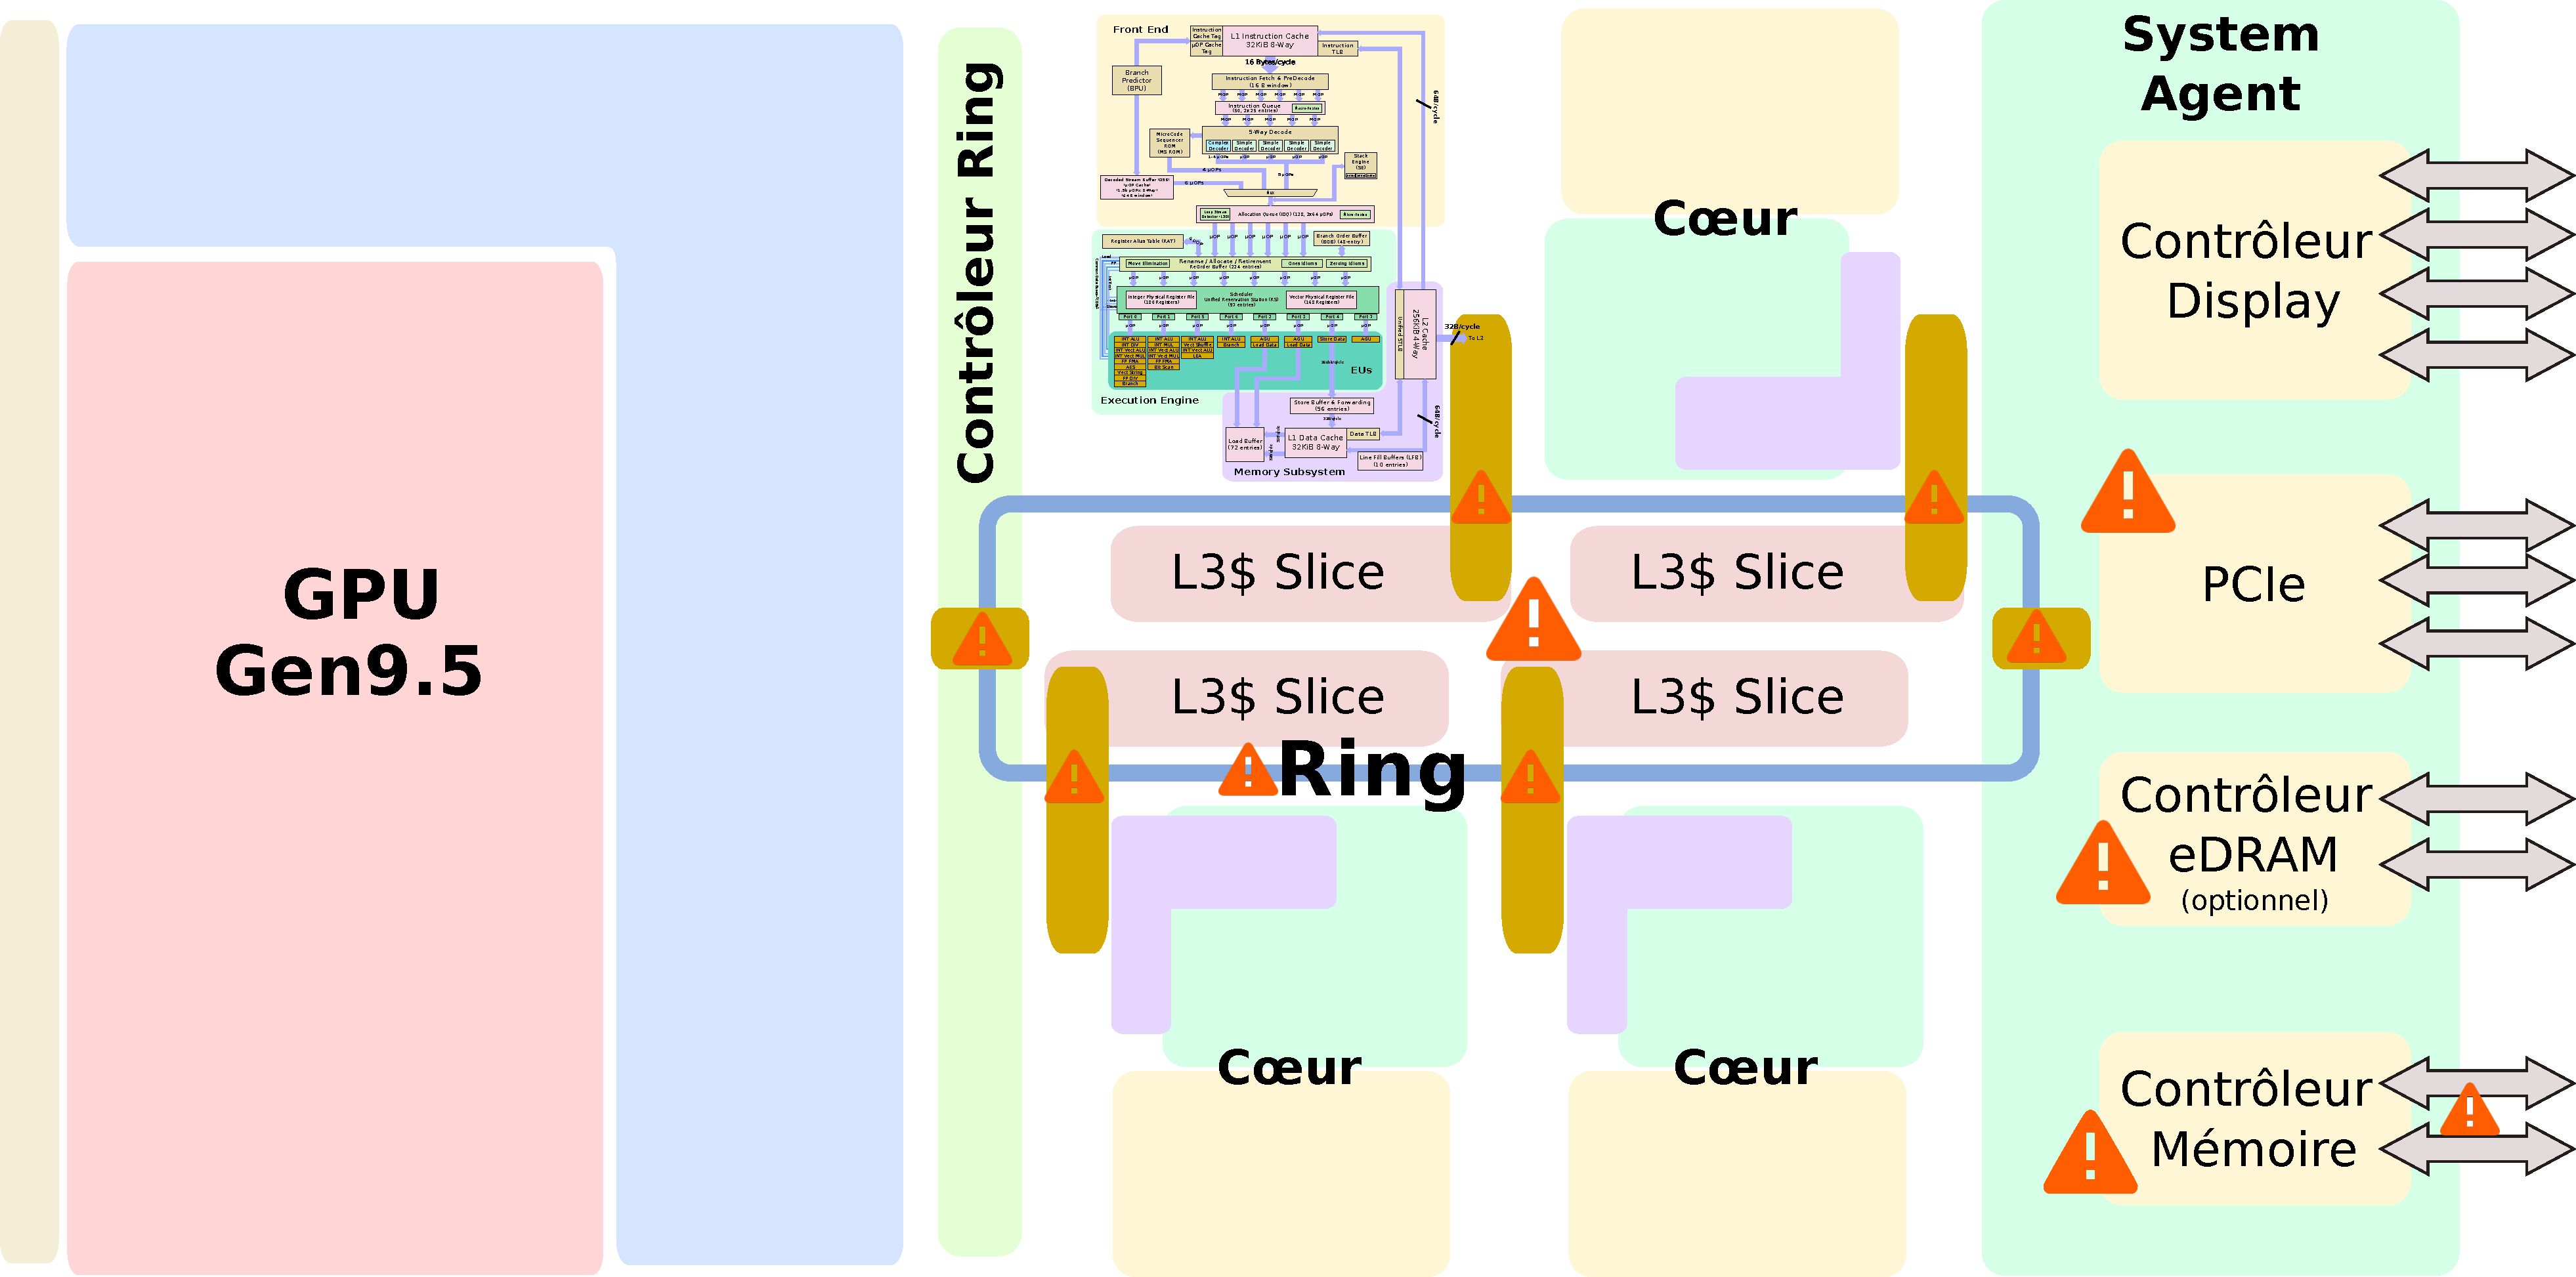
\includegraphics[width=\linewidth]{schemas/kaby_lake_soc_block_diagram}
			\captionsetup{justification=centering}
			\caption{Représentation schématique du processeur avec les points d'interférences notables}
			\label{fig:kabylakesocblockdiagram}
		\end{figure}
	
		Dans le cadre de nos expérimentations, nous établissons la fréquence de fonctionnement du processeur à une valeur fixe de 1600 MHz. L'hyperthreading est désactivé. Il s'agit d'une technologie permettant l'exécution parallèle de code sur un même cœur par dédoublement virtuel de ce dernier. Cela fait passer  le CPU de 4 cœurs physiques à 8 cœurs virtuels aux yeux du système d'exploitation. Son usage complexifie d'autant plus la gestion de l'utilisation de ressources partagées, et provoque même des partages de ressources supplémentaires, et par conséquent des sources d'interférence et donc de ralentissements d'exécution potentiels. Cela rend la maîtrise de l'exécution logicielle encore plus difficile à maîtriser par un mécanisme de contrôle et notamment pour obtenir une caractérisation représentative des interférences entre les tâches. De fait, cela nécessiterait d'observer toutes les possibilités d'exécution parallèle de code relatives à l'hyperthreading, en plus de toutes les possibilités d'exécution déjà existantes. Par conséquent, dans le cadre de notre étude et de façon plus générale, il nous semble plus pertinent de réaliser une implémentation sans utiliser de telles technologies, quitte à voir dans un second temps si leur ajout est envisageable.
		De fait, avec notre seule proposition, de nombreuses possibilités supplémentaires sont offertes en comparaison des pratiques industrielles actuelles. De ces dernières, l'on pourra citer la désactivation complète du cache qui est une pratique courante pour éviter complètement tout effet de bord non prévu par l'intégrateur du logiciel, ou encore l'usage de stratégies d'ordonnancement statiques avec des fenêtres d'exécution temporelle fixes, et potentiellement surévaluées. Ces deux éléments représentent des limitations très importantes de performances des calculateurs émergents. Ces bridages nécessaires actuellement de par un manque de maîtrise du comportement matériel, pourraient être évités avec l'utilisation de mécanismes de contrôle dynamique comme le nôtre. 
		Au regard de ce constat, il convient donc de réaliser ces études de façon progressive et donc de ne pas impliquer directement la totalité des mécanismes d'optimisation mis à disposition par les processeurs, qui apportent chacun une couche de complexité supplémentaire.
		
        \subsection{Support Logiciel}
        
        \paragraph{Système d'exploitation Linux}
        Pour mettre en application nos bancs d'essais sur cette plateforme matérielle, nous avons cherché à reprendre un système d'exploitation qui permette le plus de versatilité possible via l'utilisation d'un système Linux. L'intérêt est double. 
        
        D'une part cela offre l'opportunité de tester une grande variété de logiciels et donc de pouvoir réadapter la solution à d'autres cas et contextes d'application. Cette richesse de logiciel se traduit aussi par l'existence de librairies déjà mises à disposition et éprouvées pour nos différents besoins. On pourra mentionner la capacité de gestion de l'ordonnancement (\cite{ishkov_complete_2015}) et de l'exécution des tâches, l'automatisation des tests par scripts, des outils de stress du matériel ou encore de benchmarking (\cite{king_stress-ng_2019}) et monitoring du logiciel comme avec~\cite{girbal_metrics_2018}. Par ailleurs, plusieurs travaux ont déjà été effectués sur l'étude de Linux dans le cadre d'usage pour des systèmes temps-réel, tel que~\cite{gerum_xenomai_2004}, \cite{litayem_building_2011}, \cite{allende_towards_2019}. Ainsi, ce type de système d'exploitation est déjà largement utilisé pour des cas d'application comme en robotique~\cite{bouchier_embedded_2013} ou sur des plateforme de prototypage automobile~\cite{sivakumar_automotive_2020}, \cite{gobillot_esprit_2018}.
        
        D'autre part, l'utilisation d'une plateforme matérielle et logicielle Linux apporte un niveau de complexité supplémentaire vis-à-vis d'une plateforme industrielle usuelle, notamment au regard de la complexité du kernel impliqué. Cela se traduit particulièrement sur la politique d'ordonnancement et de gestion des tâches dans Linux comme cela a pu être couvert dans~\cite{lozi_linux_2016}. Cela présente un intérêt particulier, car si l'on arrive à obtenir des résultats probants sur l'efficacité d'un tel mécanisme de surveillance et de contrôle dans un environnement où l'on ne maîtrise pas totalement les couches bas niveau du support logiciel alors on sera en droit d'être relativement optimistes pour un usage dans des cas qui impliquent une plateforme logicielle plus focalisée sur un cas industriel. La différence principale étant d'embarquer uniquement le logiciel dans un cas réel contrairement à un choix de test comme une distribution Linux grand public qui implique déjà un certain nombre de tâches et de drivers qui s'exécutent en fond. 
        
        Nous nous baserons plus spécifiquement sur une distribution Linux Mint XFCE, version 20.04, avec un kernel en version 4.15.8.
        
        \paragraph{Co-kernel Xenomai}
        De façon à utiliser Linux dans le cadre d'applications temps-réel, nous y adjoignons Xenomai~\cite{gerum_xenomai_2004} en version 3.1. Il s'agit d'un co-noyau qui se patche au noyau de base Linux de façon à lui apporter des fonctionnalités propres au développement d'applications temps-réel. Cela apporte notamment de meilleures performances en termes de latence comparé aux appels système Linux natif. Cela est dû au fait qu'initialement, le noyau Linux présente une grande part de code qui est non-préemptif. En conséquence, l'exécution de code non critique peut retarder la gestion d'interruptions destinées à exécuter du code temps-réel. Les différentes solutions de modification du noyau comme Xenomai, ou encore le patch \texttt{preempt-rt} dans une moindre mesure, répondent directement à cette problématique pour diminuer au mieux la latence constatée. Les écarts de latences observées sur la gestion des interruptions de l'ordre de millisecondes sont réduites à des microsecondes avec Xenomai. Les différentes solutions qui modifient Linux pour tenter d'y apporter un meilleur cadre d'utilisation de logiciel temps-réel ont pu être comparés dans~\cite{brown_how_2010}. 
        
        Le choix que nous avons fait a été déterminé aussi du fait qu'il fournit un framework complet pour exécuter des tâches temps-réel avec une gestion de tous les outils relatifs au domaine : \begin{itemize}
        	\item sémaphores et mutex,
        	\item protocoles d'envoi/réception de données entre tâches,
        	\item ordonnancement et allocation de tâches avec périodicité,
        	\item gestion d'alarmes et interruptions,
        	\item gestion d'entrée/sortie en évitant des latences propres à Linux.
        	\end{itemize}
    	De plus, ce framework est disponible suivant différentes interfaces de développement. Cela facilite la portabilité d'une application entre différents frameworks temps-réels et le framework Xenomai natif. Ainsi, il est possible d'exécuter sur un support Xenomai du logiciel utilisant les interfaces de POSIX, PSOS, RTAI (qui est le prédécesseur de Xenomai), \textmu-ltron, VRTX, VxWorks et rtdm avec peu de modification du logiciel. Par ailleurs, notre choix de cette combinaison d'une carte mère basée sur un processeur Intel avec Xenomai est confortée par le fait qu'Intel ait déjà étudié la question de l'usage de Xenomai sur ses calculateurs multicœur~\cite{intel_corporation_hard_2009}. Ce framework sera utilisé pour l'implémentation du mécanisme de surveillance et contrôle.
    	
    	De façon générale, ce qui permet à Xenomai d'offrir toutes ces fonctionnalités avec des latences réduites en cohabitation avec le noyau Linux réside dans l'ajout d'une couche \texttt{Adeos}~\cite{gerum2005life} qui est un pipeline des  interruptions. Il permet la préemption de toutes les interruptions système pour les distribuer en priorité vers le domaine Xenomai avant tout envoi de ces dernières vers le domaine Linux. Cela inclut à la fois les interruptions matérielles et logicielles, ainsi que tous les envois de signaux système (changement d'état d'une tâche pour la mettre en pause/démarrer/arrêter, mutex etc.). Cela priorise \textit{de facto} l'exécution de code du domaine Xenomai et réduit au maximum les latences dues au noyau Linux. La différence entre un noyau Linux simple et avec un patch Xenomai est représenté en ~\autoref{fig:architecturekernel}. On constate que le co-noyau propose un équivalent symétrique aux composants natifs du noyau Linux, il s'agit 

		\begin{figure}[h]
			\centering
			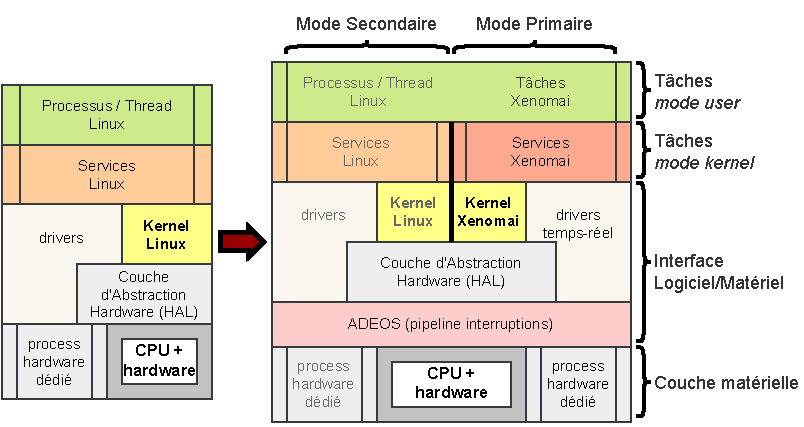
\includegraphics[width=\linewidth]{schemas/Architecture_kernel}
			\caption[Architecture co-noyau Linux et Xenomai]{Architecture du noyau Linux et avec patch Xenomai}
			\label{fig:architecturekernel}
		\end{figure}
    	
		Il est à noter qu'au sein des systèmes Linux, ce que l'on nomme "\textit{tâche}" est désigné sous le nom de processus ou de thread. La différence fondamentale entre ces deux appellations étant que chaque processus possède son propre espace mémoire virtuel, tandis que les threads peuvent se partagent un espace mémoire virtuel commun s'ils sont lancés à partir d'un même processus parent. Du point de vue de l'ordonnancement du système d'exploitation, threads et processus sont équivalents. Cette différence sur la mémoire est, en ce qui nous concerne, négligeable. En effet, il s'agit bien de mémoire \textit{virtuelle}, c'est-à-dire que du point de vue des processus ils disposent d'un espace mémoire réservé, mais dans les faits il s'agit de mémoire physique qui est partagée. Le contrôleur mémoire du système d'exploitation étant responsable de la mise en correspondance entre adresses mémoires virtuelles et espaces mémoires physiques. Ainsi, que l'on travaille avec des threads ou des processus, les risques d'interférences par usage de ressources partagées tel que les cache reste identique. On continuera à parler de "tâches" par la suite.
		
		Il existe deux modes d'exécution des tâches sur un système Linux~:  en mode User ou Noyau, que l'on peut retrouver sur les 2 couches supérieures de l'architecture logicielle de la~\autoref{fig:architecture}. Dans le mode Noyau, les tâches ont les droits pour exécuter des instructions privilégiées. Cette distinction est importante, car les opérations bas niveau que nous devons employer pour la surveillance et la gestion d'ordonnancement des tâches nécessite l'emploi d'instructions privilégiées. Avec l'utilisation de Xenomai s'ajoute une nouvelle dimension. Les tâches peuvent alors s'exécuter soit dans le domaine Xenomai en mode Primaire, soit dans le domaine Linux en mode Secondaire. L'avantage principal du domaine Xenomai étant la faible latence d'exécution, proche d'un système temps-réel dur. En revanche si une tâche dans ce domaine requiert des appels système Linux, alors une migration vers le domaine Linux est nécessaire. Xenomai réalise cela par un mécanisme de \textit{shadowing} où la tâche est clonée dans le domaine Linux dit mode "secondaire" pour effectuer les appels systèmes nécessaires. La transition entre les modes se fait de façon fainéante" (\textit{lazy mode switch}) dans le sens où  un changement de mode n'est fait qu'au moment où un appel de fonction requiert d'être dans l'autre mode de fonctionnement. 
		
		Si nous relevons cette spécificité logicielle, c'est parce que chaque changement de mode engendre un surcoût de temps d'exécution. Par conséquent, une tâche qui utiliserait successivement des appels système Linux et des fonctionnalités Xenomai bas-niveau peut très vite engendrer un très fort surcoût d'exécution. Dans les fonctionnalités de Xenomai sont inclus la gestion de mutex, de signaux ou autres appels aux APIs temps-réel de Xenomai (gestion d'ordonnancement, alarme, interruptions...). C'est d'ailleurs pour cette raison qu'au fil du temps un bon nombre d'appels système ont eu droit à un équivalent dans les API de Xenomai, pour éviter un passage en mode secondaire. C'est le cas par exemple des fonctions de récupération des \texttt{timers}. De façon plus générale, la correspondance entre les différents domaines applicatifs de Xenomai est un aspect très important de son développement pour permettre le plus facilement possible une inter-compatibilité entre les différents systèmes temps-réel et Linux. Une bonne part des enjeux et des méthodes déployées pour l'implémentation d'un système temps-réel donné sous Linux est développé dans~\cite{gerum_xenomai_2015}. 
	    Suivant ce constat, dans le cadre de l'utilisation d'un jeu de tâche arbitraire pour la réalisation de nos tests, nous devons être vigilants sur l'utilisation d'appels système et du nombre de changements de mode. Des tâches ayant de mauvais résultats sur ces métriques (notamment un surplus de changement de modes) sont probablement inadaptés à représenter des tâches temps-réel, à moins d'être modifiées spécifiquement pour éviter ce problème. 


        
        %~\cite{wong_towards_2008}, \cite{lelli_efficient_2011} %% scheduling
        %We used Linux (Linux Mint xfce 18.04 distribution) to mix general purpose and real-time applications with different scheduling policies (\cite{wong_towards_2008}, \cite{lelli_efficient_2011}). Its versatility grants easier compatibility with benchmarking suites. Moreover, by adding Xenomai (v. 3.1) real-time co-kernel~\cite{gerum_xenomai_2004}, it is possible to get closer to real-time applications with latencies lowered from milliseconds down to microseconds. It also grants an API for real-time application development, used for the MCA framework.
                        
		%Notably, POSIX enables to force tasks execution to dedicated cores and change both priority and scheduling policy. As we are in a controlled context that suppose no malicious behavior, we do not implement mechanisms like memory protection or strong space isolation policies. As stated before, vanilla Linux Kernel is not made for hard real-time application. That is mainly because kernel is not preemptive on most parts of it, this can cause high latency for real-time interrupts, from kernel code execution that could be linked to non-critical applications. % due to its non-preemptiveness. It causes high latencies to the system due to kernel and drivers interrupts.
        %Therefore, we add a Xenomai co-kernel to improve latency down to micro-seconds and run our MCA to respect desired real-time constraints.
        %Please note that from Linux point of view, ``threads" and ``processes" are equivalent and correspond to ``tasks" for us.
            
                        Threads are assigned 2 parameters, a scheduling policy and a static priority (\textit{sched\_priority}). Both are considered by the global scheduler. It first gathers the threads by priority level to execute highest priority processes first. Then for a same priority level, the scheduling policy of each task will define which one to run first. For normal processes the priority level is ignored (considered at 0) to be executed following the CFS policy. This way, a real-time process with a priority level from 1 (lowest) to 99 (highest), always run before them. The threads' scheduling policy defines how they are inserted into the list of same priority level and how they move in this list, all processes being preemptive.  We can list 3 real-time policies for real-time process: FIFO, EDF and Round-Robin. \\
                        For this purpose, Linux allows to bound threads to cores. For a processor with $j$ cores, every thread has a core affinity represented by an array of $j$ Booleans. Each of these Booleans of affinity $b_{Ti}$ indicates if the thread $T$ can be executed on the core $i$. By default, every normal process has a core affinity of $\begin{pmatrix}1 & 1 & 1 & 1\end{pmatrix}$, for a quad-core processor, meaning that it can be executed by every core. It makes it easier for the scheduler to balance load between every core. But for our case and when it comes to run hard real-time applications, it is interesting to use such affinity. This way, it will be possible to isolate our MCA on an isolated core and bound the benchmark processes to the other threads.
        %Xenomai is a real-time kernel that can be installed as a co-kernel to a classic Linux distribution as presented in deep by \cite{gerum_xenomai_2004}. Our framework and experiments are implemented on the real-time APIs proposed by Xenomai 3.1.
            %in order to implement it and add measurements instrumentation. %Xenomai version installed is 3.0.5, from tutorial \cite{hoarau_beta_2017}.
        %In such configuration, it adds an interruption pipeline (ADEOS) directly between the hardware and OS low-level software (i.e. Hardware Abstraction Layer, OS Kernel and drivers). This enables to catch all the interrupts and distribute them in priority to Xenomai real-time kernel.
        %Threads executed with Xenomai are executed either in primary or secondary mode. In both cases they are memory-protected from other processes. By default, Xenomai threads starts in primary mode. They get directly access to Xenomai API and are scheduled by its real-time scheduler. A Xenomai thread can however use kernel API with system calls. When it happens, the Xenomai tasks goes temporarily to the Linux scheduler and automatically goes back to Xenomai domain once done. As the priority system used on primary mode is compatible with the secondary one, the Xenomai tasks keep their highest priority status. It makes the mode switch transparent.
            
        %All things considered, we mainly use Xenomai to get a significant latency gain (divided by up to 10) for the critical tasks. We can stay on the classic Linux domain for our non-critical tasks.
            
        Such OS configuration allows us to specify a per-task core allocation and priority level. Linux scheduler as explained in~\cite{ishkov_complete_2015} selects tasks first by priority level, (from 1 to 99 for real-time tasks domain). Then for a given priority level, multiple scheduling policies are possible: Global Earliest Deadline First, FIFO, Round-Robin, and other best-effort policies. To test a system using classic Round-Robin for instance, every task are launched at same priority level with Round-Robin policy. We use Rate-Monotonic scheduling policy for our tests this way.
                        
    \section{Benchmark MiBench}
        \subsection{Présentation}
        MiBench~\cite{guthaus_mibench_2001} est un benchmark qui a été développé par Guthaus \& al.~\cite{guthaus_mibench_2001} dans l'idée de proposer une librairie d'applications qui couvrent un large panel de domaines. Nous l'utilisons de façon à pouvoir en sélectionner des tâches pour représenter au mieux un cas d'application réaliste. 
        Ce benchmark dispose de codes source classifiés en 6 domaines d'application : automobile, réseau, utilisateur, bureautique, sécurité et télécoms. Dans chaque domaine plusieurs tâches sont proposée, chacune d'entre elle en deux versions, "petite" et "grande", qui représente en relativement plus ou moins de temps d'exécution (notamment via la taille de la donnée d'entrée, quand il s'agit d'un traitement d'image par exemple). Au total, ce sont plus de 30 tâches, chacune en version "petite" et "grande" donc. Le résumé des tâches de ce benchmark est présenté dans la~\autoref{tab:mibench_tasks} .
        
\begin{table}[ht!]
	\centering
	\caption{Tâches MiBench}
	\label{tab:mibench_tasks}
	\begin{tabular}{@{}llll@{}}
		\toprule
		Nom          & Description                                  & Type d'entrée      & Type de sortie         \\ \midrule
		bitcount     & comptage de bits	vers entiers        & texte ASCII        & texte ASCII         \\
		qsort        & algorithme de tri                    & texte ASCII        & texte ASCII         \\
		susan c      & reconnaissance de coins              & image (.pgm)       & image (.pgm)        \\
		susan e      & reconnaissance de bords              & image (.pgm)       & image (.pgm)        \\
		susan s      & lissage d'image (réduction de bruit) & image (.pgm)       & image (.pgm)        \\
		jpeg c       & encodeur JPEG                        & image (.ppm)       & image (.jpeg)       \\
		jpeg d       & décodeur JPEG                        & image (.jpeg)      & image (.ppm)        \\
		lame         & encodeur MP3                         & audio (.wave)      & audio (.mp3)        \\
		mad          & décodeur audio MP3                   & audio (.mp3)       & audio (.wave)       \\
		tiff2bw      & conversion en noir et blanc          & image (.tiff)      & image (.tiff)       \\
		tiff2rgba    & conversion couleurs RGB en TIFF		& image (.tiff)      & image (.tiff)       \\
		tiffdither   & tramage noir et blanc (dithering)    & image (.tiff)      & image (.tiff)       \\
		tiffmedian   & réduction de plage de couleur      	& image (.tiff)      & image (.tiff)       \\
		dijkstra     & recherche de plus court chemin		& texte ASCII        & texte ASCII         \\
		patricia     & recherche sur arbre PATRICIA			& texte ASCII        & texte ASCII         \\
		ghostscript  & interpréteur PostScript              & PostScript		 & image (.ppm)        \\
		ispell       & Vérificateur orthographique          & texte              & texte ASCII		   \\
		rsynth       & synthèse vocale de texte             & texte              & audio (.AU)         \\
		strgsearch & recherche de mot dans un texte			& texte              & texte               \\
		blowfish d   & déchiffrement blowfish               & données (bin.)  	 & données (bin.)      \\
		blowfish e   & chiffrement blowfish                 & texte              & données (bin.)      \\
		pgp d        & déchiffrement asymétrique      		& données (bin.)  	 & texte               \\
		pgp e        & chiffrement asymétrique				& texte              & données (bin.)      \\
		rijndael d   & déchiffrement AES                    & données (bin.)  	 & texte               \\
		rijndael e   & chiffrement AES                      & texte              & données (bin.)      \\
		sha          & algorithme de calcul de hash			& texte              & texte ASCII         \\
		adpcm c      & encodeur de PWM                      & audio (.wave)      & données (bin.)      \\
		adpcm d      & décodeur de PWM                      & données (bin.)  	 & données (bin.)      \\
		CRC32        & somme de contrôle 32 bits     		& audio (.wave)      & texte ASCII         \\
		gsm          & encodage GSM                         & audio (.AU)        & données (bin.)      \\ 
		\bottomrule
	\end{tabular}
\end{table}
    
        Those tasks do different jobs similar to ones in these domains, with different levels of complexity that is of high interest for us.

            To run an artificial system load as a ``worst-case" cache, memory, CPU use and I/O stress, we use Linux \textit{Stress-ng} tool presented in~\cite{king_stress-ng_2019}. 


            As we do not have yet real industrial application for testing, for now the MiBench Benchmark suite~\cite{guthaus_mibench_2001} has been used for our experiments. The objective is to use applications similar as much as possible to computation profiles that could be found in real applications, in order to reproduce memory containment and resource usage close to real cases. 
            %We lack real applications to test, but 
            
            MiBench consists of a large panel of tasks with different memory needs and execution profiles to mimic existing applications. We have at disposal applications from 5 different domains, as presented in the \autoref{MiBenchTable}. It is used here to validate the framework and put into practice our experiments.\\
            \begin{table}[!t]
                %% increase table row spacing, adjust to taste
                \renewcommand{\arraystretch}{1.3}
                % if using array.sty, it might be a good idea to tweak the value of
                %\extrarowheight as needed to properly center the text within the cells
                \caption{tâches MiBench retenues}
                \label{MiBenchTable}
                \centering
                %% Some packages, such as MDW tools, offer better commands for making tables
                %% than the plain LaTeX2e tabular which is used here.
                \begin{tabular}{|c||c|}
                    \hline
                    Automotive  & basicmath, bitcount, qsort, susan (smooth/edges/corners)\\
                    \hline
                    Network     & dijkstra, patricia                                        \\
                    \hline
                    Consumer    & jpeg (code \& decode), typeset                            \\
                    \hline
                    Office      & stringsearch                                              \\
                    \hline
                    Security    & blowfish, rijndael, sha                                   \\
                    \hline
                    Telecom     & adpcm (coding \& decoding), CRC32, FFT, FFT\up{-1}, gsm               \\
                    \hline
                \end{tabular}
            \end{table}
            We selected a set of 16 applications from MiBench for our experiments. Most of them exists in ``small" and ``large" version that allows to change proportionally their execution time and resource needs. Also, some of these tasks may have several variants according to setup parameters. For instance, $Sunsan$ has 6 different variants: edge detection, corner detection and smoothing, all 3 existing in both ``small" and ``large" version which works with a bigger image for processing. This way, those 16 applications leads to 45 different possible tasks for our experiments. It enables to test different combination following the ``size" and number of tasks but also the kind of tasks we use.
            Tasks profile classification were already made by Guthaus \& al. in~\cite{guthaus_mibench_2001} and detailed work about their memory consumption can be found in~\cite{blin_understanding_2016}. 
        
        \subsection{Demandes d'adaptation/modification des tâches}
    \section{Agent de Monitoring et Control}
            \begin{figure}
                \centering
                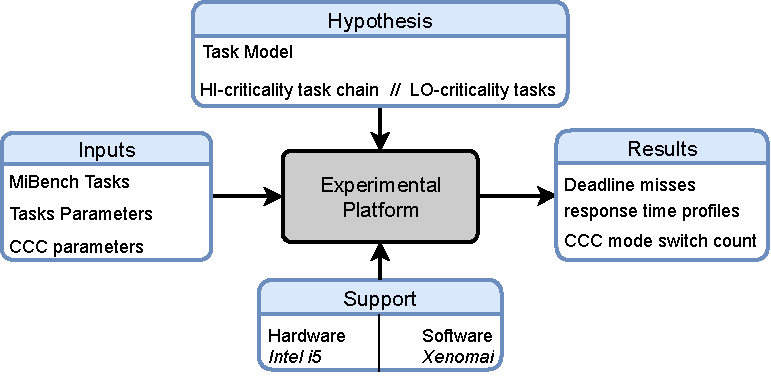
\includegraphics[width=\linewidth]{ExperimentsArch}
                \caption{Experimental Platform structure\label{fig:expe}}
            \end{figure}
    
%\chapter{Bilan de l'expérimentation}
    \section{Solutions adoptées à la complexité d'implémentation}
        Difficultés rencontrées dans la mise en place de ce concept et leçons apprises (en cas de volonté de reproduction)

\ifdefined\included
\else
\bibliographystyle{StyleThese}
\bibliography{these}
\end{document}
\fi